\chapter{@Arquitetura}\label{arquitetura}

@Explicação da arquitetura do projeto

% https://www.sharelatex.com/blog/2013/08/29/tikz-series-pt3.html
\begin{figure}[!htp]
    \centering
    \begin{tikzpicture}[node distance=2cm,on grid,auto]

    \node (inicio) [startstop] {Início};
    \node (proc1) [process, below of=inicio] {Processo 1};
    \node (fim) [startstop, below of=proc1] {Fim};

    \draw [arrow] (inicio) -- (proc1);
    \draw [arrow] (proc1) -- (fim);

    \end{tikzpicture}
    \caption{Arquitetura da aplicação}
    \label{arquitetura-da-aplicação}
\end{figure}

Conforme a arquitetura da aplicaçao~\ref{arquitetura-da-aplicação}...

\begin{figure}
  \centering

  \begin{sequencediagram}
    \newthread{ss}{}{SimulationServer}
    \newinst{ctr}{}{SimControlNode}
    \newinst{ps}{}{PhysicsServer}
    \newinst[1]{sense}{}{SenseServer}

    \begin{call}{ss}{Initialize()}{sense}{}
    \end{call}
    \begin{sdloop}{Run Loop}
      \begin{call}{ss}{StartCycle()}{ctr}{}
        \begin{call}{ctr}{ActAgent()}{sense}{}
        \end{call}
      \end{call}
      \begin{call}{ss}{Update()}{ps}{}
        \begin{call}{ps}{PrePhysicsUpdate()}{sense}{state}
        \end{call}
        \begin{callself}{ps}{PhysicsUpdate()}{}
        \end{callself}
        \begin{call}{ps}{PostPhysicsUpdate()}{sense}{}
        \end{call}
      \end{call}
      \begin{call}{ss}{EndCycle()}{ctr}{}
        \begin{call}{ctr}{SenseAgent()}{sense}{}
        \end{call}
      \end{call}
    \end{sdloop}
  \end{sequencediagram}

  \caption{UML sequence diagram demo.}
\end{figure}

\begin{figure}
  \centering

  \begin{sequencediagram}
    \newthread{ss}{}{SimulationServer}
    \newinst{ps}{}{PhysicsServer}
    \newinst[1]{sense}{}{SenseServer}
    \newthread[red]{ctr}{}{SimControlNode}

    \begin{sdloop}[green!20]{Run Loop}
      \mess{ctr}{StartCycle}{ss}
      \begin{call}{ss}{Update()}{ps}{}
        \prelevel
        \begin{callself}{ctr}{SenseAgent()}{}
          \begin{call}[3]{ctr}{Read}{sense}{}
          \end{call}
        \end{callself}
        \prelevel\prelevel\prelevel\prelevel
        \setthreadbias{west}
        \begin{call}{ps}{PrePhysicsUpdate()}{sense}{}
        \end{call}
        \setthreadbias{center}
        \begin{callself}{ps}{Update()}{}
        \end{callself}
        \begin{call}{ps}{PostPhysicsUpdate()}{sense}{}
        \end{call}
      \end{call}
      \mess{ss}{EndCycle}{ctr}
      \begin{callself}{ctr}{ActAgent()}{}
        \begin{call}{ctr}{Write}{sense}{}
        \end{call}
      \end{callself}
    \end{sdloop}

  \end{sequencediagram}

  \caption{Example of a sequence with parallel activities.}
\end{figure}

% https://tex.stackexchange.com/questions/207240/drawing-simple-sequence-diagram
\begin{figure}
  \centering
    \scalebox{1}
    {  \begin{sequencediagram}
    \newthread{A}{\shortstack{Cliente\\ \\\begin{tikzpicture}
\node [copy shadow,fill=gray!20,draw=black,thick ,align=center] {Aplicaciones \\ Cliente};
\end{tikzpicture}}}{}
    \newinst[1]{B}{\shortstack{Servidor de \\ aplicaciones \\ \\ 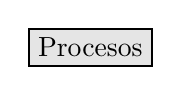
\begin{tikzpicture}
\node [fill=gray!20,draw=black,thick ,align=center] {Procesos};
\end{tikzpicture}}}{}
    \newinst[1]{C}{\shortstack{Servidor de \\  de Datos \\ \\\begin{tikzpicture}[shape aspect=.5]
\tikzset{every node/.style={cylinder, shape border rotate=90, draw,fill=gray!25}}
\node  at (1.5,0) {BD};
\end{tikzpicture}}}{}
    \begin{call}{A}{}{B}{}
    \end{call}
    \begin{call}{B}{}{C}{}
    \end{call}
  \end{sequencediagram}
  }
\caption{Arquitectura en 3 capas}
\end{figure}